\documentclass{standalone}
\usepackage{tikz}
\begin{document}
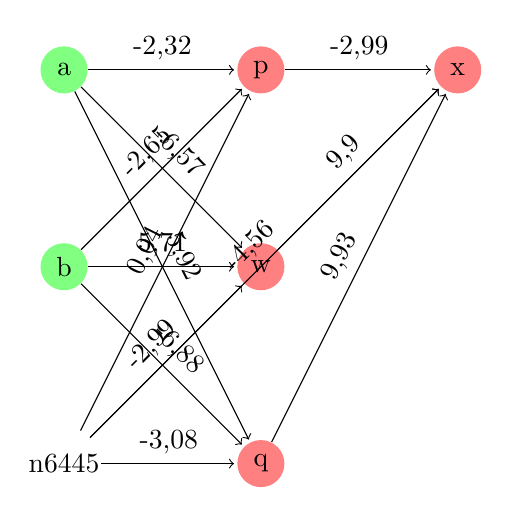
\begin{tikzpicture}[shorten >=1pt,->,draw=black!,node distance=2.5cm]
\tikzstyle{neuron}=[circle,fill=black!25,minimum size=17pt,inner sep=0pt]
\tikzstyle{constant}=[neuron, fill=white!50];
\tikzstyle{sigmoid}=[neuron, fill=red!50];
\tikzstyle{identity}=[neuron, fill=green!50];
\node [identity] (a) {a};
\node [identity,below of=a] (b) {b};
\node [constant,below of=b] (n6445) {n6445};
\node [sigmoid,right of=a] (p) {p};
\node [sigmoid,below of=p] (w) {w};
\node [sigmoid,below of=w] (q) {q};
\node [sigmoid,right of=p] (x) {x};
\path[every node/.style={sloped,anchor=south,auto=false}]
(n6445) edge node {-2,99} (w)
(n6445) edge node {-3,08} (q)
(n6445) edge node {-4,56} (x)
(n6445) edge node {0,04} (p)
(p) edge node {-2,99} (x)
(w) edge node {9,9} (x)
(q) edge node {9,93} (x)
(b) edge node {-6,88} (q)
(b) edge node {5,71} (w)
(b) edge node {-2,65} (p)
(a) edge node {5,92} (q)
(a) edge node {-6,57} (w)
(a) edge node {-2,32} (p)
;\end{tikzpicture}
\end{document}